\subsection{Параллельный коррелятор}

Программные приемники системы Navstar GPS рассмотрены в \cite{tsui, akos-book}.
После стадии детектирования сигнала, оценка частоты для заданного источника поступает в модуль уточнения частоты.
Уточненная частота и фаза ПСП поступают в ФАПЧ.

Одним из параметров системы ФАПЧ является шумовая полоса.
Этот параметр определяет количество теплового шума попадающего в систему ФАПЧ. Широкая шумовая полоса позволяет системе ФАПЧ быстро войти в синхронизм,
но также ведет к существенному ухудшению характеристик системы ФАПЧ за счет возрастания уровня теплового шума.

Область синхронизации частоты, в пределах которой обеспечивается срыв синхронизация, при ${\zeta>0.3}$ определяется как \cite{spilker-book}:

\begin{center}
\begin{equation}
	\label{eq:corr_pll_band}
	\Delta \omega_m = 2 \omega_n (\zeta + 0.6)
\end{equation}
\end{center}
где ${\omega_n}$ - собственная частота системы ФАПЧ, ${\zeta}$ - коэффициент демпфирования,

Примем ${\zeta=0.707}$. Данное значение ${\zeta}$ близко к оптимальному \cite{tsui, spilker-book}, тогда ${\Delta \omega_m = 2.614 \omega_n}$.
Собственная частота системы ФАПЧ вычисляется по формуле:

\begin{center}
\begin{equation}
	\label{eq:corr_pll_freq}
	\omega_n = \frac{8 \zeta B_L}{4 \zeta^2 + 1} 
\end{equation}
\end{center}
где ${B_L}$ - шумовая полоса.

Традиционный подход детектирования сигнала предусматривает корреляцию входного сигнала и набора локальных копий сигнала шагом 1 кГц.
Для стационарного приемника Navstar GPS диапазон смещения частоты обусловленный Допплеровским эффектом \cite{tsui} может находится в диапазоне ${\pm 5}$ кГц.
Таким образом, для получения оценки с точностью 1 кГц необходимо провести поиск в 11 ячейках. В каждой ячейке намнеобходимо ${N}$-комплексных умножений.
Для наземных приемников типовое значение  ${B_L=20}$ Гц \cite{tsui, akos-book}. Область синхронизации из выражения \ref{eq:corr_pll_band} и  \ref{eq:corr_pll_freq}.
${\Delta \omega_m \approx 100}$ Гц. Таким образом необходима стадия уточнения частоты.

Схема традиционного приемника изображена на рисунке \ref{pic:corr_scheme}.
\begin{figure}[H]
	\center\scalebox{1}{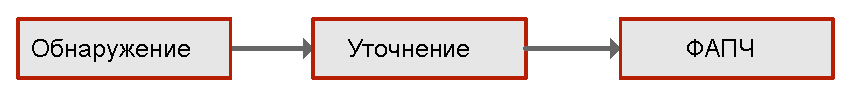
\includegraphics[width=1\linewidth]{corr_scheme.eps}}
	\caption{Схема традиционного приемника}
	\label{pic:corr_scheme}
\end{figure}

Количество комплексных умножений, требуемых для оценки частоты одного источника параллельным коррелятором: ${OP_{FFT} = 12NlogN + 11N}$

Алгоритм уточнения частоты описан в \cite{tsui}. Следует отметить, что данный алгоритм основан на усреднении фазы и требует дополнительной оперативной памяти
(ОЗУ) приемника для хранения 5 миллисекунд данных при обработке одного источника. Оперативная память потребляет значительное количество энергии,
поэтому снижение количества необходимой ОЗУ является важной задачей при разработке портативных приемников.
Так же обработка 5 мс данных повышает встретить переход бита внутри данных – это ведет к дополнительным сложностям при реализации программных приемников сигнала Navstar GPS.

Количество умножений, требуемых для уточнения частоты одного источника: ${OP_{FINE} = }$

\newpage
